% !TeX document-id = {a7325568-63cb-46d1-95d6-777a45054e5a}
% !TeX TXS-program:compile = txs:///pdflatex/[--shell-escape]
\documentclass{article}
\usepackage{style}
\begin{document}
\maketitle
\tableofcontents
\section{Introducción}
La red de Hamming es una red de tipo sin supervisión, su objetivo es calcular la distancia de Hamming entre los vectores prototipo y los de entreda para encontrar la distancia mínima, se conforma dos capas:
\begin{enumerate}
	\item Capa FeedFoward
	Esta capa realiza el producto interno, entre cada uno de los prototipos y el patrón de entrada sumado con el vector de bias, después se le aplica una función de transferencia lineal.
	\item Capa Recurrente
	Esta capa también es conocida como la capa competitiva, las neuronas de esta capa son inicializadas  con las salidas de la capa feedfoward, en esta capa las neuronas ``compiten'', al terminar solo una neurona tendrá una salida diferente de zero, lo que indica en que categoría está el prototipo de entrada.
\end{enumerate}
El objetivo de la red es decidir cual vector prototipo está más cercano al vector de entrada.
\newpage
\subsection{Modelo}
\begin{figure}[h!]
	\caption{Modelo}
	\centering
	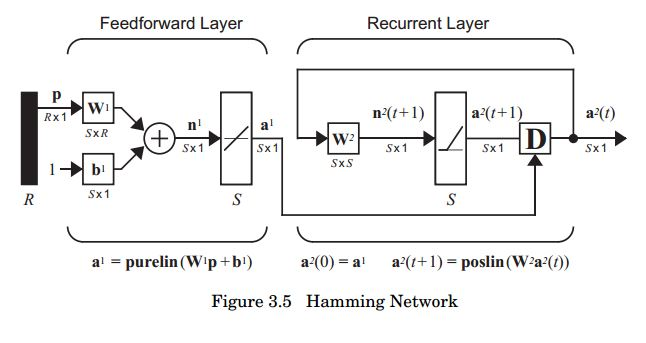
\includegraphics{modelo}
\end{figure}
\newpage
\section{Diagrama de Flujo}
\begin{figure}[htpb]
	\centering
	\includesvg[width = 400pt, height = 400pt]{diagram}
	\caption{Diagrama de Flujo}
\end{figure}
\newpage
\section{Resultados}
\subsection{Ejemplo 1}
\begin{lstlisting}
	Ingrese la matriz de los valores prototipos. 
	Las columnas separados por espacios y las filas con ;  
	(e.g. 1 2 3;4 5 6;7 8 9)
	>>> 1 -1 -1;1 1 -1
	Ingrese el vector de entrada. Los valores separados por espacios (e.g. 1 2 3)
	>>> -1 -1 -1
	El vector de entrada pertenece a la clase: 1
	Vector final:
		3
		0
\end{lstlisting}
\begin{figure}[htpb]
	\centering
	\includesvg[width = 400pt, height = 400pt]{r1}
	\caption{Gráfica del ejemplo 1}
\end{figure}
\newpage
\subsection{Ejemplo 2}
\begin{lstlisting}
	Ingrese la matriz de los valores prototipos. 
	Las columnas separados por espacios y las filas con ;  
	(e.g. 1 2 3;4 5 6;7 8 9)
	>>> 1 -1 -1 1;1 -1 1 -1;-1 1 1 -1;-1 1 -1 -1
	Ingrese el vector de entrada. Los valores separados por espacios (e.g. 1 2 3)
	>>> -.7 -.1 .2 -.5
	El vector de entrada pertenece a la clase: 3
	Vector final:
		0
		0
		1.1904
		0
\end{lstlisting}
\begin{figure}[htpb]
	\centering
	\includesvg[width = 400pt, height = 400pt]{r2}
	\caption{Gráfica del ejemplo 2}
\end{figure}
\newpage
\section{Discusión de Resultados}
Para cada uno de los resultados se muestra:
\begin{enumerate}
	\item A cual categoría más se acercó el vector de entrada (solo si convergió).
	\item El vector final ($a^2(t)\ \ \text{donde}\ \  0 \leq t \leq 40$) (solo si convergió).
	\item La gráfica del ``historial'' de la evolución de $a^2$ (solo si convergió).
	\item Si convergió o no.
\end{enumerate}
\section{Conclusiones}
La red de Hamming es una red interesante, ya que, usa dos capas(FF y recurrente) fue creada para separar patrones dado su vector de entrada, el número de neuronas son igual en las dos capas. Fue una gran aportación para el campo de las redes neuronales. Aprendí nuevas cosas investigando la teoría y práctica(matlab), fue divertida e interesante.
\section{Referencias}
Martin T Hagan. Machine Learning, Neural Network Design (2nd Edition), 2014.\\
\url{http://home.agh.edu.pl/~vlsi/AI/hamming_en/}
\section{Apéndice}
\begin{lstlisting}[
style=Matlab-editor,
basicstyle=\mlttfamily,
escapechar=`,
caption={Código},
]
% Datos ingresados por el usuario
proto_prompt = ['Ingrese la matriz de los valores prototipos. ' ...
'Las columnas separados por espacios y las filas con ;  (e.g. 1 2 3;4 5 6;7 8 9)\n'];
cell_arr = regexp(input(proto_prompt, 's'),';','split');
p = str2num(input('Ingrese el vector de entrada. Los valores separados por espacios (e.g. 1 2 3)\n', 's'))';
% Capa Feed Foward
W1=[];
for i=1:length(cell_arr)
	% Agregar la columna "parseada" nueva al final de la matriz
	W1 = [W1; str2num(cell_arr{i})];
end
n = size(W1, 1);
b1 = ones(n,1) * size(W1, 2);
a1 = W1 * p + b1;
% Capa Recurrente
epsilon = 1 / n;
W2(1:n, 1:n)=-epsilon;
W2(1:n+1:end)=1;

% Condiciones Iniciales
a2 = a1;
h_values = []
h_values = [h_values;a1'];
a2 = poslin(W2*a2);
% Valores Extra
h_values = [h_values; a2'];
tries = 40;
winners = 0;
has_converged = false;
% Iteraciones
for i = 1:tries
	has_winner = find_winner(a2);
	if(has_winner)
		winners = winners + 1;
	else
		has_winners = 0;
	end
	if(winners == 2)
		has_converged = true;
		break;
	end
	a2 = poslin(W2*a2);
	h_values = [h_values; a2'];
end

if (has_converged)
	for proto = 1:length(a2)
		if (a2(proto) > 0)
			fprintf('El vector de entrada pertenece a la clase: %d\n', proto);
			fprintf('Vector final:\n');
			disp(a2);
			break;
		end
	end
	plot(0:i, h_values');
else
	fprintf("La red no convergió\n");
end

% Función para encontrar las neuronas encendiades en el vector a
function [is_winner] = find_winner(vector)
	counter = 0;
	for i = 1:size(vector, 1)
		if(vector(i) > 0)
			counter = counter + 1;
		end 
	end
	if counter ~= 1
		is_winner = false;
	else
		is_winner = true;
	end
end
\end{lstlisting}
\end{document}